\chapter{Data Analysis I: Calibration and Corrections}

Need to explain pedestal subtraction 
GG noise subtraction 

\section{Software}

The S$\pi$RITROOT software is modular tasked based code based on the FAIRROOT package written in C++ \cite{fairroot}. The main tasks in the S$\pi$RITROOT software reconstruction are:
\begin{itemize}
  \item Decoder task
  \item Pulse Shape Algorithm (PSA Task)
  \item Helix Track Finding Algorithm
  \item Clustering Algorithm
  \item Track Fitting (GENFIT package)
  \item Vertex Fitting (RAVE package)
\end{itemize}

The decoder task converts the binary data file into a container class which maps the electronics channels into the corresponding pads and (x,z) coordinates. 

There may be several pulses in a pad coming from two tracks passing under the same pad separated  by arrival time. Using an expected pulse shape the PSA task fits the signal pulses within a pad, giving the arrival time of the drifted electrons from each particular track. The height of the fitted pulse is proportional to the total charge of that event, Q and the y-coordinate is calculated as $y = v\cdot t_0$ where $v$ is the drift velocity and $t_0$ the arrival time. Combining the information from these first two tasks, (x,y,z,Q), we construct what is called a "hit". 

 The Helix Track Finding Algorithm finds the collection of hits belonging to one track out of all the hits in an event. The hits within a track are then reduced into clusters. A cluster's position is the average position of the hits within a cluster, with the total charge of the cluster being the sum of the hits charges. 
 
 A tracks average position is estimated by the cluster's average position. The clusters are then fitted in the GENFIT track fitting package \cite{genfit}, giving the final momentum of the track. A final vertex of the event is fitted from all tracks using the package RAVE \cite{rave}. 

\paragraph{Definition of clustering}

A brief description of the method of clustering is illustrated in Figure \ref{fig:topview}. It is impractical to cluster in both the x and z-axis and we only cluster the hits along one axis. The three clusters at the bottom of Figure \ref{fig:topview} are clustered along the x-axis and the upper three are along the z-axis, as shown by the bolded pads for one of the clusters in each direction.

 The clustering direction depends on the angle  of the track with respects to the x-axis, defined as $\theta$. For example, a track going along the z-axis the crossing angle is defined as $90^{\circ}$, and a track going along the x-axis defined as $0^{\circ}$. In the case that the crossing angle is $45^{\circ} < \theta \leq 90^{\circ} $ the clustering direction is along the x-axis. For $0^{\circ} < \theta \leq 45^{\circ}$ it is along the z-axis. 

 The position along the clustering direction is calculated by weighting the individual hit's positions by their charges $q_i$ and getting the mean value. The other direction is set to the center of the pad. For example if we are clustering along the x-axis for a cluster, the z-position is set to the center of the pad in the z-direction and vice versa. 

Clustering in this way gives us better position resolution for calculating the position of each cluster. You could imagine if we calculated the clusters only along the x-axis for tracks with $\theta \approx 0^{\circ}$ the x-position is not well defined. By clustering in the direction most perpendicular to the track, we get a better position resolution.

\begin{figure}[H]
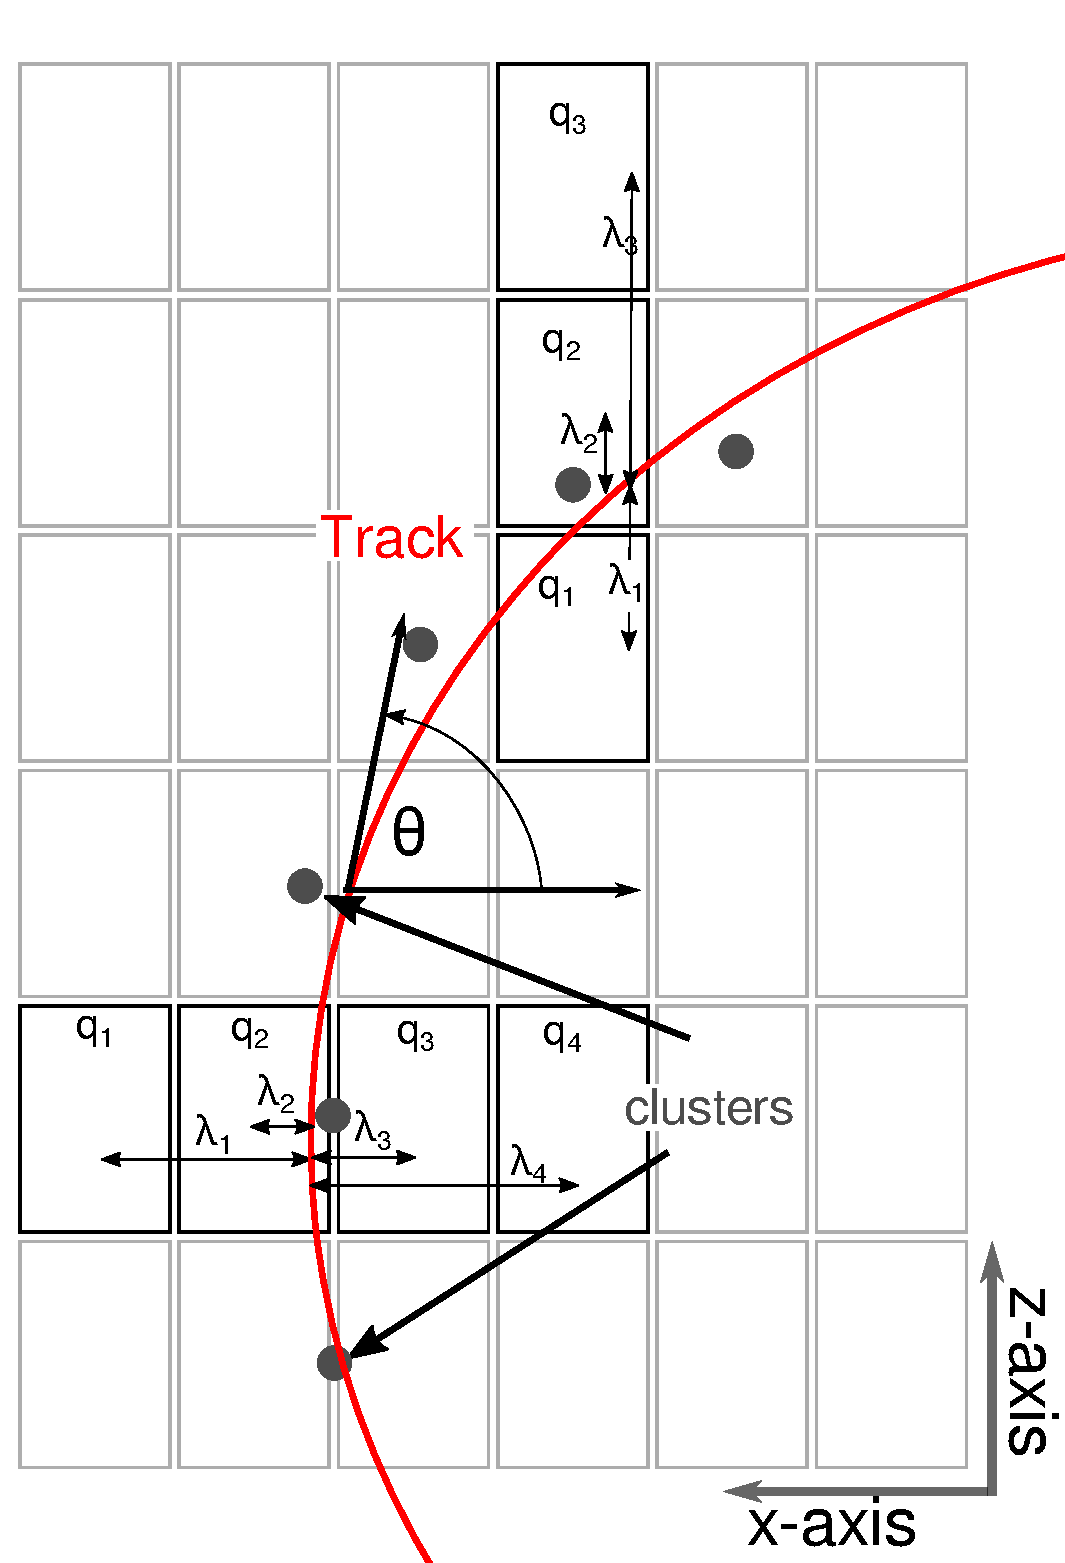
\includegraphics[scale=.5]{top_view_helix_ext.pdf}
\caption{Cartoon graphic of a top down view of a fit to a track passing through several pads. The bolded pads and the charges $q_i$ represent the hits belonging to that pad and the clusters of the track representing the average position of the track. The three clusters at the bottom are clustered in the x-direction and for the upper three clustered in the z-direction. The estimate of the position of the avalanche is given by the track fit and the position from the center to each pad to the $\bar{x}$ position is given as $\lambda_i$.}
\label{fig:topview}
\end{figure}

\begin{figure}[H]
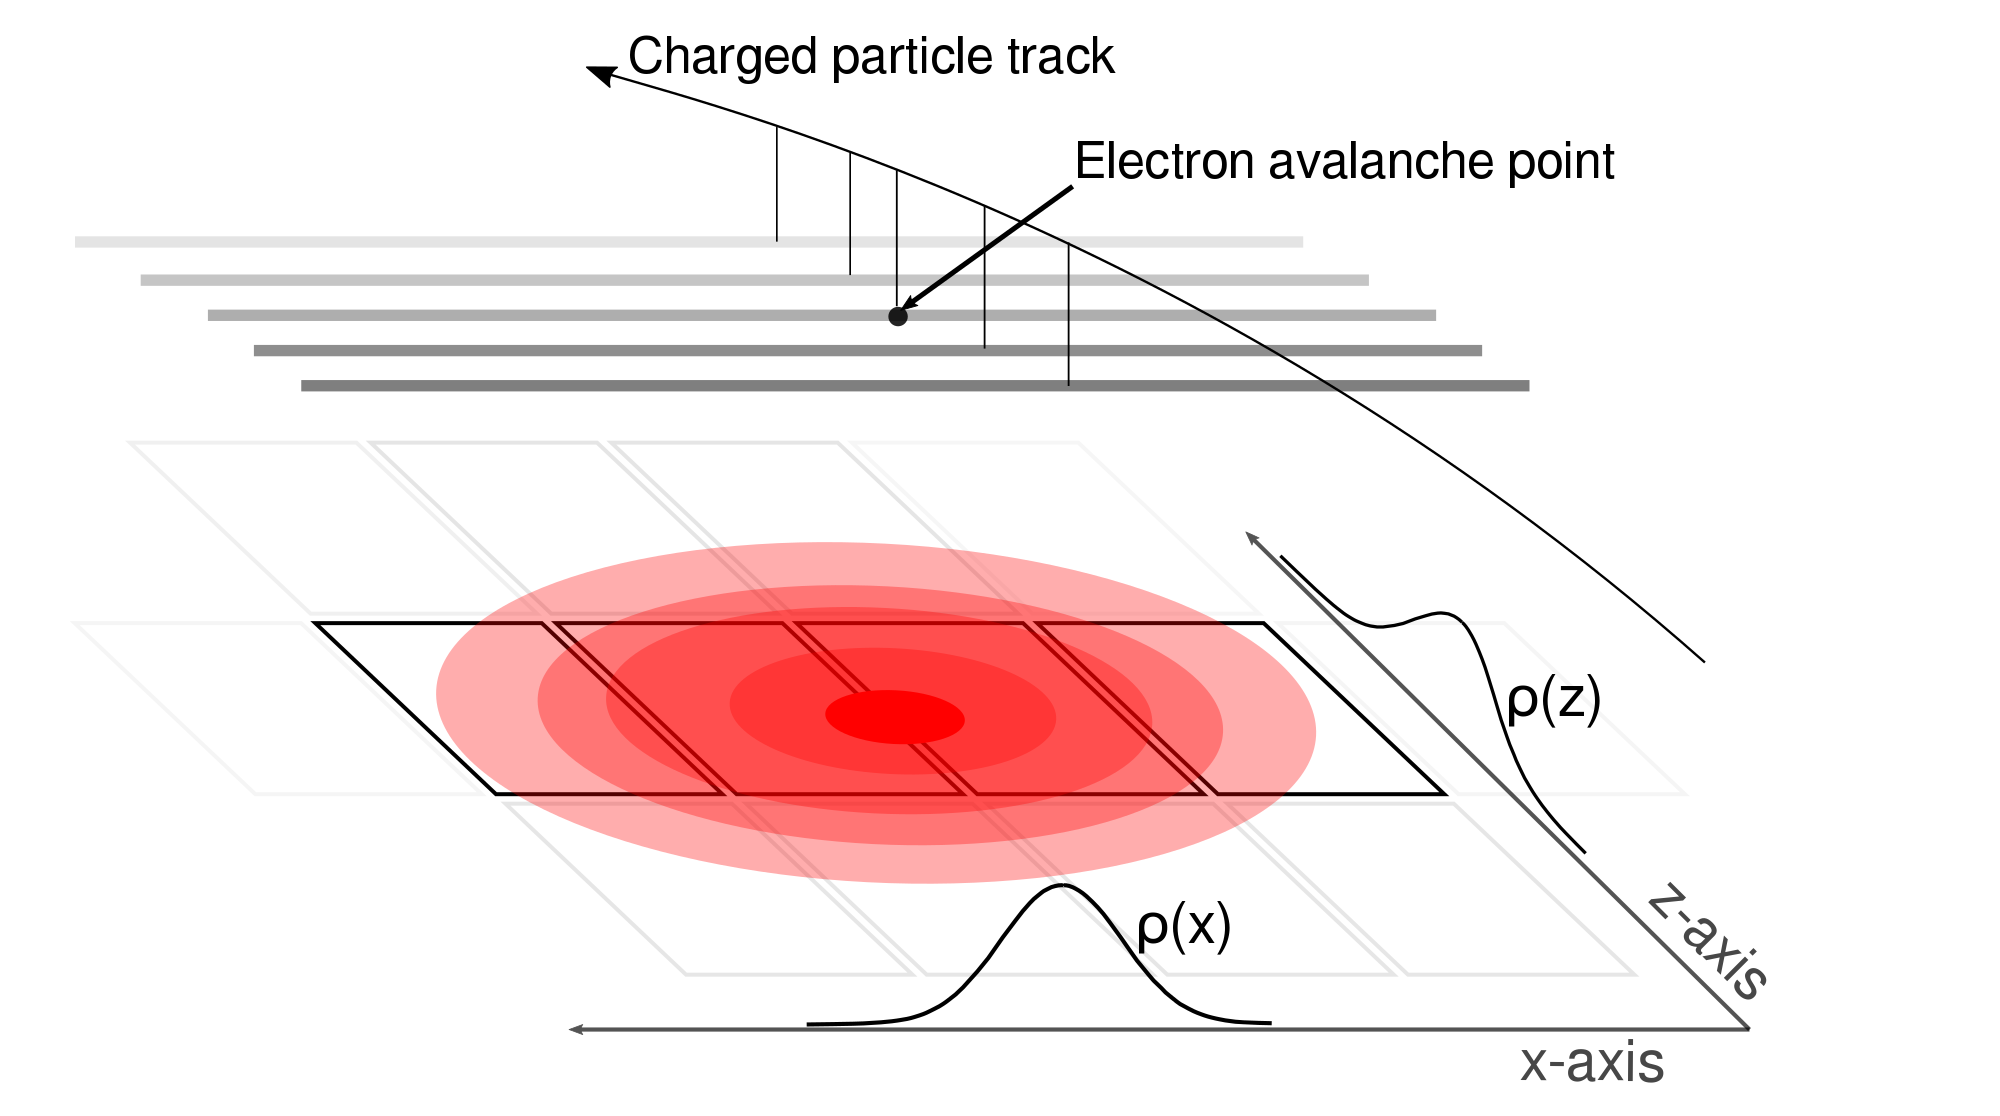
\includegraphics[width=\linewidth]{padsat_Large}
\caption{A cartoon illustration of the charge distribution resulting from an electron avalanche on one wire and the projections of the distribution onto the two axis $\rho(x)$ onto the x-axis and $\rho(z)$ onto the z-axis. The orientation of the wire planes is flipped upside down to display the perspective better.}
\label{fig:prf}
\end{figure}



\section{Calibrations and Corrections}


\subsection{Cocktail calibration}

\begin{table*}\centering
\ra{1.3}
\begin{tabular}{@{}rrrrcrrrcrrr@{}}\toprule
& \multicolumn{3}{c}{$100 MeV$} & \multicolumn{3}{c}{$100 MeV$} & \multicolumn{3}{c}{$300 MeV$}\\
\cmidrule{2-4} \cmidrule{6-8} \cmidrule{10-12}
& &\multicolumn{2}{c}{Measured} & & \multicolumn{2}{c}{Measured} & & \multicolumn{2}{c}{Measured}\\
\cmidrule{3-4} \cmidrule{7-8} \cmidrule{11-12}
Particle &\phantom{abc} & Raw & E$\times$B\\
\midrule
p   & 882.8 & d & d & 903.5 & e & e &\phantom{abcdef} & f & f \\
d   & 817.1 & d & d & 898.5 & e & e & 1621.1 & f & f\\
t   & 589.5 & d & d & 887 & e & e & 1612.4 & f & f  \\
$^{3}$He  & 1617.3  & d & d & 1795.2 & e & e & 3236.4 & f & f\\
$^{4}$He  & 1405.6  & d & d & 1782.9 & e & e & 3226.4 & f & f \\
\bottomrule
\end{tabular}
\caption{Summary of expected cocktail. }
\label{tb:cocktailsummary}
\end{table*}

Cocktail Calibration 
Picture of cocktail before and after ExB effect
Table of LISE++ expected cocktail energies ridigity setting of dipole magnets (reference big rips line)



\subsection{Electronics calibration}
Pulse the ground grid. 
\begin{figure}[H]
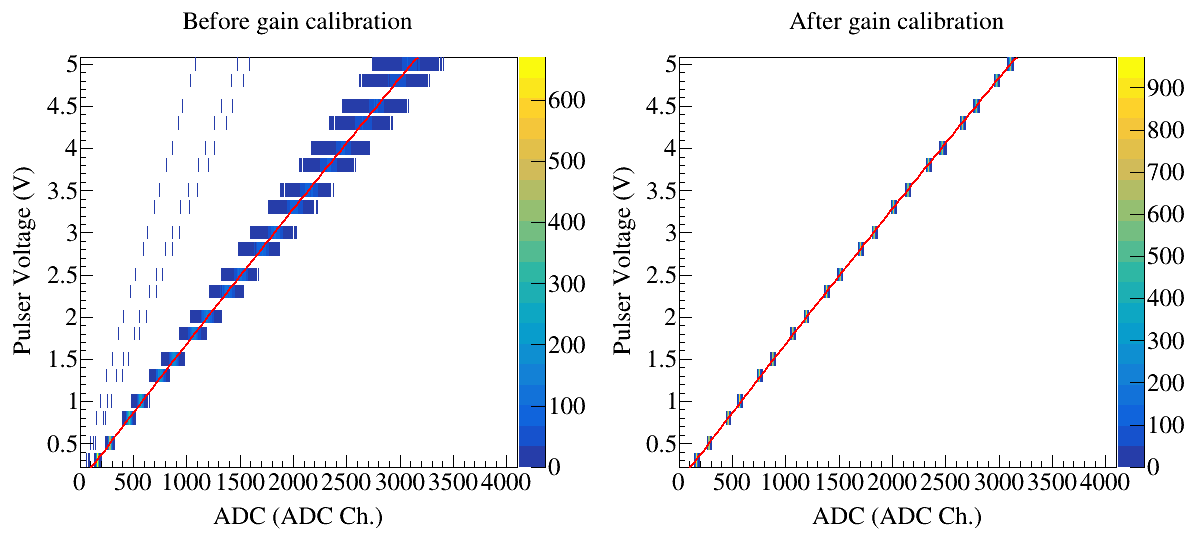
\includegraphics[width=\linewidth]{gaincalib.png}
\caption{Calibration of electronics}
\label{fig:gaincalib}
\end{figure}

\subsection{Anode gain calibration}

\begin{figure}[H]
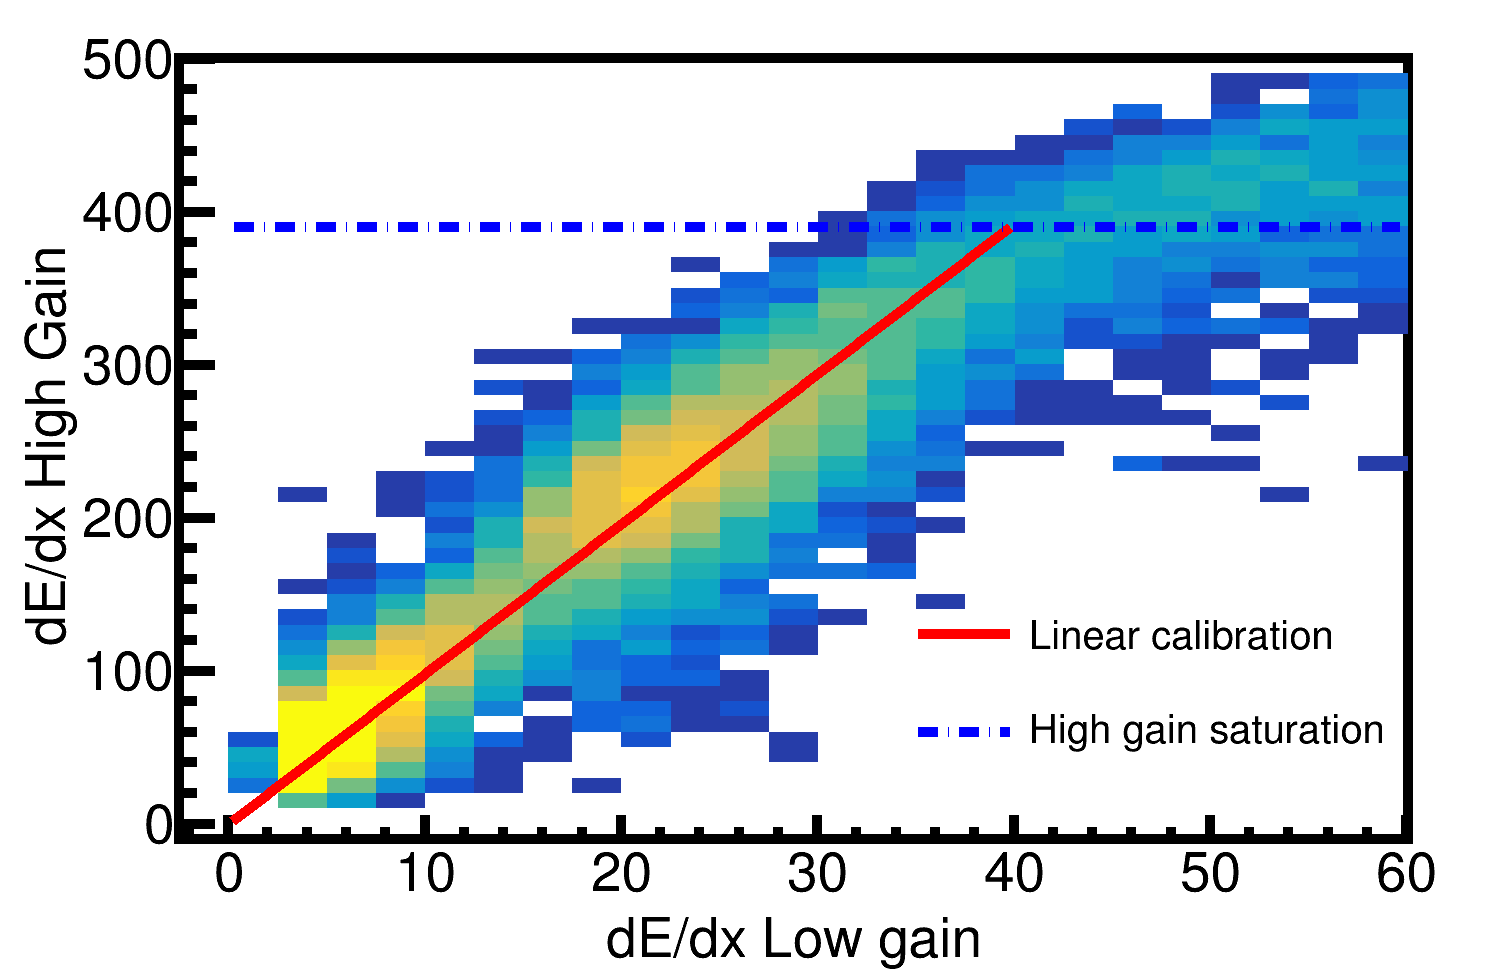
\includegraphics[width=\linewidth]{highlowcal.png}
\caption{Calibration of low high.}
\label{fig:highlowcal}
\end{figure}

Picture of low vs high gain channels and fit

\subsection{Extending the dynamic range of the Electronics}
Add paper here. 

\subsection{Space Charge Corrections}
Overview
Discuss the relevant time scales, drift lengths, magnitudes, and locations of space charge

\begin{figure}[H]
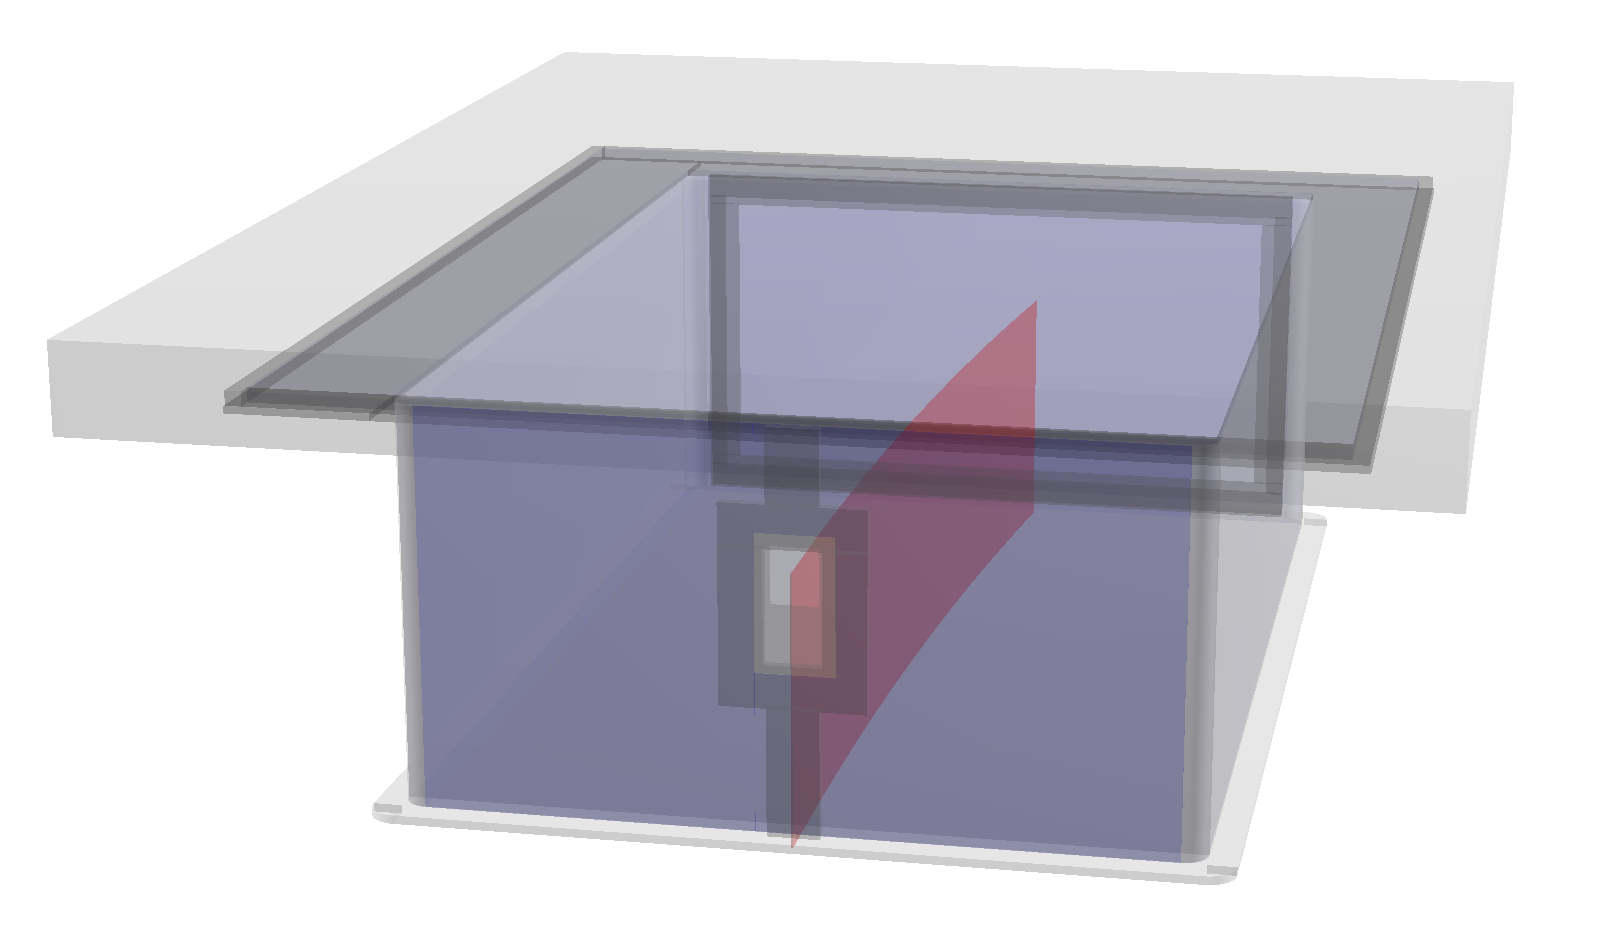
\includegraphics[width=\linewidth]{spacechg_cartoon.png}
\caption{Location of space charge in 132 Sn}
\label{fig:spacechg_cartoon}
\end{figure}

\begin{figure}[H]
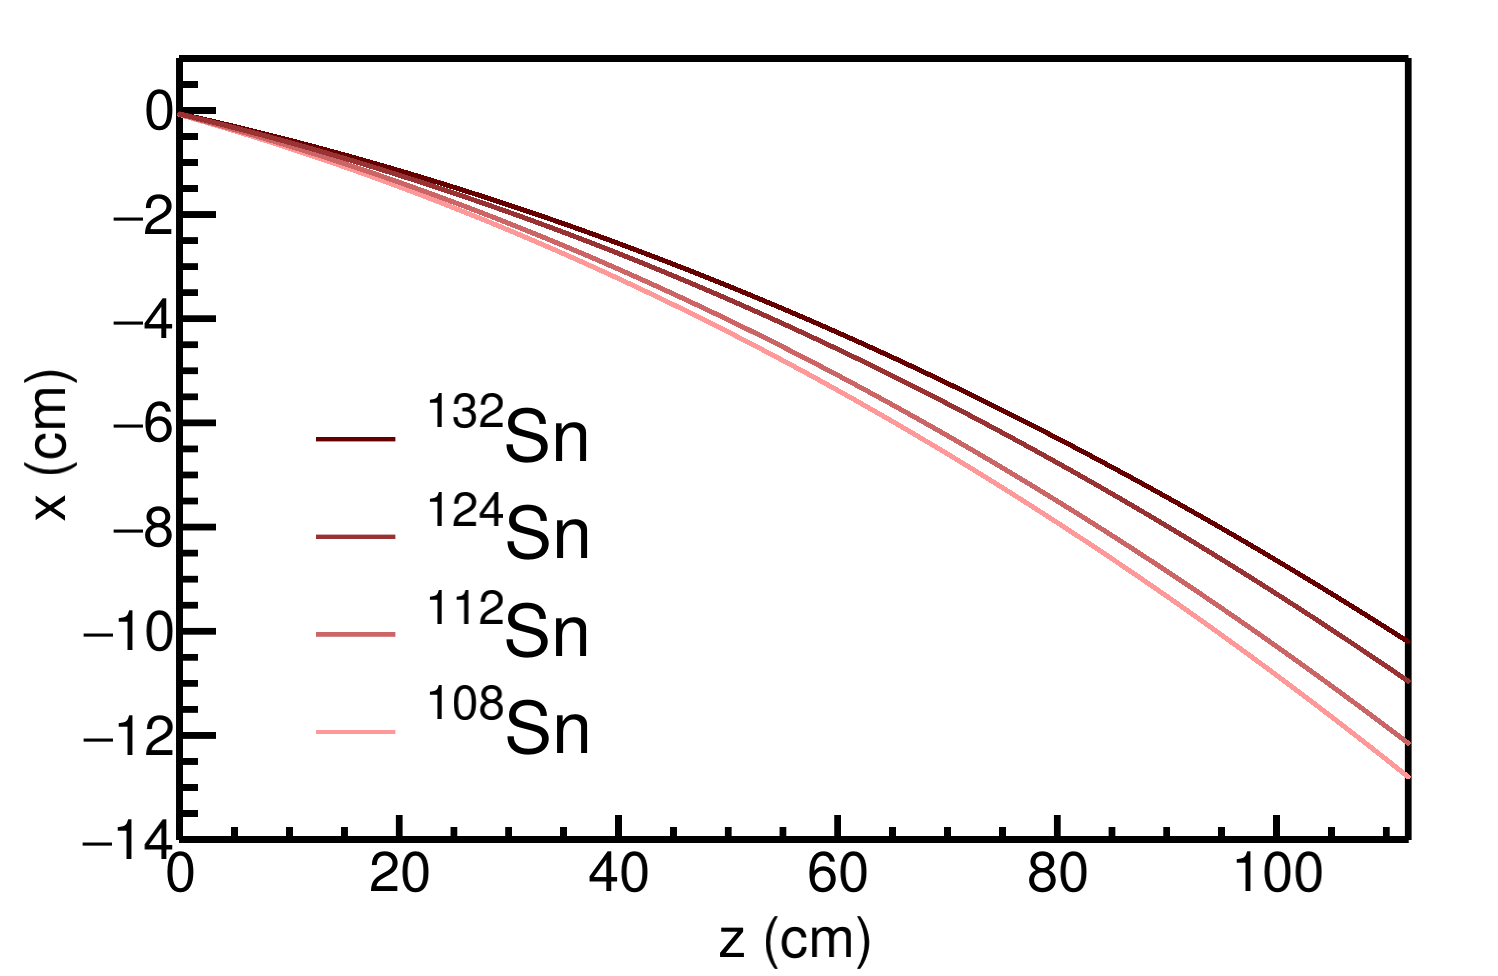
\includegraphics[width=\linewidth]{beampath.png}
\caption{Beam path of the experiments}
\label{fig:beampaths}
\end{figure}


\begin{table}[!htp] % not just 'h!'
\centering % not a center environment
\begin{tabular}{
  @{}
  l
  S[table-format=1.2]
  S[table-format=1.2]
  S[table-format=1.2]
  S[table-format=5.2]
  S[table-format=5.2]
  @{}
}
\toprule
Beam Energy Loss  &
 {${}^{132}$Sn} &
 {${}^{124}$Sn} &
 {${}^{112}$Sn} &
 {${}^{108}$Sn} &
  {Avg.}\\
  
\midrule
$\si{\kilo\eV\per\centi\meter}$ & 11.2   &.034  &5.43   &  903   &150     \\
\bottomrule
\end{tabular}

\caption{Average energy loss of each beam.}
\label{tb:beameloss}
\end{table}

Reference appendix for poisson solver 
Tables for ion drift velocity in P-10 Gas reference Sauli
Figure of sDAC or POCA 
Figure of cartoon of what is happening to tracks
Figure of correction map in TPC and MC map 
Figure of before and after correction BDC vs reco momentum
Figure of track residuals before and after?


In theory, a TPC functions with the electric and magnetic fields parallel to each other. In this way the electrons move opposite to the electric field winding tightly around the magnetic field lines, reducing transverse diffusion in the process. In practice, due to the finite size of the dipole magnet and field cage, there are traverse components to both the electric and magnetic fields. These transverse components introduce drift velocities in the transverse directions, causing a shift in the measured cluster positions of the track. Thereby introducing systematic shifts in the calculation of the momentum and the vertex calculation. 

Most of the time the beam does not undergo a nuclear collision with the target and passes through the TPC drift volume. The KATANA array threshold was set to veto such events, ensuring the gating grid remain closed to prevent the large amount of charge deposited by the beam into the avalanche region. While the electron drift velocity is fast enough for the electrons produced by the unreacted beam to terminate on the closed gating grid, the drift velocities of the positive ions produced are of order $10^{-4}$ times slower. At higher beam rates the positive charge is allowed to pile up producing a region of positive space charge, introducing perturbations to the nominal electric field. 

Since the beam comes in along the z-axis, and the drift direction of the ions is in the -y direction, we can estimate the charge density as an uniform sheet charge. The surface charge density is related to the beam rate, ion drift length, ion drift velocity, and the energy loss of the beam. Though the incoming beam comes randomly, the slow drift velocity combined with the high beam rate makes the uniform approximation valid. Tracking or estimating the beam rate as a function of time with in a given run would provide a better estimate of the space charge. Or experimentally a laser system could be pulsed after each event (throughout the drift volume), giving the experimental correction map for the drift. While the potential for a laser system was implemented in the field cage design, a laser system ultimately was not developed for the \spirit tpc. 

The beam rate within a run is roughly constant, therefore we can estimate the space charge and provide a first order correction for the space charge effect. 

As mentioned in CHAPTER ???, the cocktail beam momentum was well known to within 1\% as set by the BIGRips spectrometer. Also time of flight analysis of upstream and downstream scintilators also independently confirmed the beam rigidity setting. The expected momentum is given in TABLE ??? as calculated by from the beam rigidity setting of the magnet (WHICH MAGNET). The measured momenta as determined by the TPC software (given in FIG TABLE ), shows a disagreement on the level of 5\% too high. We noticed that if one only uses the first 90 layers (out of 112) of the TPC, the momenta is lower; one should expect the momentum to go higher as the track length is shorter (short tracks effectively are straight lines). 
In the cocktail beam there is no un-reacted beam causing any significant space charge. The magnetic field map of the SAMURAI magnet has been calculated by TOSCA simulation CITE ???, and several points have been verified experimentally with a hall probe to be within XXX \%. We assume that the electric field (to first order) is uniform in the y-direction. Using Garfield++ CITE ???, we can model the transverse drift of the electrons in the presence of such fields. 

A grid of electrons uniformly distributed in the TPC model space were drifted to the gating grid position. The final shifts in the x and z positions was measured. 


\section{Monte Carlo Simulation}
We use Geant4 as and event generator for performing Monte Carlo Simulations in the TPC. A scale model of field cage, front window, front window frame, pad plane, and aluminum top plate are modeled. The correct materials are used as well as the field cage is modeled with P-10 gas at a density of ????. By using Geant4 we can also input the the magnetic field map of the SAMURAI dipole magnet (as calculated by the SAMURAI group via a TOSCA simulation).  In this way any particle type may be studied and the full interactions (scattering, decay, energy loss, path taken, etc.), are accounted for. The output of this simulation is a series of energy loss points which contain the amount of energy lost in $keV/cm$ and the position in $(x,y,z)$.

Separate software tasks model the converting energy loss into electrons, the drifting of electrons, the avalanche process, and the electronics response.

\begin{figure}

\includegraphics[scale=.01]{place}
\caption{A summary of all the effects modeled in the TPC MC simulation.}
\label{fig:place}
\end{figure}

\subsection{Drift Task}
The drift task takes the energy loss points calculated from Geant4 and converts them into electrons.  and then modeling their drift behavior in the field cage. As discussed previously the various processes[CITE To formula about drifting electronc]


 A full microscopic treatment of the stochastic nature of each electron would be too cumbersome; most of the properties of the electrons are described by macroscopic quantities can be described by 
The charge of each MC point is converted to the total number of electrons liberated in the P-10 gas. This is a well understood property of proportional counters and is stable over a wide range of velocities and particle types [CITE BOOK]. The conversion factor of P-10 can be calculated by considering the partial volumes of each component of the gas.  \ref{eq:kev2el}.

\begin{equation}
Number of e^{-} = 28 keV/cm
\label{eq:kev2el}
\end{equation}

\subsection{Pad Response Task}
After the avalanche process of the previous task, the total charge of the event is split over several pads defined by the Pad Response Function (as discussed in section ????). As shown in Fig.~\ref{fig:onepad}, there are three wires that lie directly above a given pad. The $z$ coordinate of the avalanche can only be one of these three wires, where as the $x$ coordinate can be any value along the wire. The functional form of the software PRF (given in Eq.~\ref{eq:softPRF}), was tuned to match the experimental data. Shown in Fig.~\ref{fig:mcdataPRF}, we see the tuned software PRF can match the experimental PRF from data over several crossing angles (as mentioned in Chapter ???? governs the shape of the PRF). 

\begin{equation}
PRF(x,z) = \frac{1}{2\pi\sigma_z\sigma_x}\exp^{\frac{-{(x-x_o)}^2}{2\sigma_x^2}}\exp^{\frac{-{(z-z_o)}^2}{2\sigma_z^2}}
\label{eq:softPRF}
\end{equation}

\begin{figure}

\includegraphics[scale=.005]{place}
\caption{A cartoon of the wires over one pad. }
\label{fig:onepad}
\end{figure}

\begin{figure}

\includegraphics[scale=.005]{place}
\caption{Comparison of MC and data PRF}
\label{fig:mcdataPRF}
\end{figure}

\subsection{Electronics Task}
The electronics task takes the total charge on each pad and simulates the electronics response, converting electronics into ADC channels. Accounting for the pedestal, the measured output in ADC channels (for a given gain setting) is given in Eq.~\ref{eq:etoADC}.

\begin{equation}
\mathrm{1 ADC }= \frac{ADC_{\mathrm{Max}} - ADC_{\mathrm{Pedestal}}}{G*f_c}
\label{eq:etoADC}
\end{equation}

\subsection{Simulating Saturation}
Add figure showing saturated time bucket spectra with location of saturation identified and with pulse shape from embedding I would like to add and how it blocks it.
Add Figure with 2D pad plane response with and without saturation flag


\section{Monte Carlo Track Embedding}
Add Figure of MC track embedding 



Track embedding is the process of taking a simulated MC track from Geant4 and embedding its response into a real data event. After reconstructing this new embedded event we match the input MC track embedded to its corresponding final reconstructed track.  By doing so we can evaluate the response of the entire TPC system to any given input value. The TPC system is composed of three major components (each which can introduce errors and or biases) the software, the detector, and the experimental setup.  

As discussed in [SOFTWARE CHAPTER] the software is composed of several task, each which introduce some error. Table {REF TABLE] listing some of the errors each task may introduce illustrating how difficult propagating the errors would be through each system. 

The detector system itself introduces errors related to the physical processes of the measurement itself. To address this we model the TPC (and its materials) in a Geant4 simulation which provides an accurate description of various interactions of a particle traversing the materials (including the gas volume) of the TPC. 


 software is the most straight forward; let the software routine process an input and measure the result. Understanding the measurement requires modeling the physics involved in the theory and operations of TPC's and the  electronics. The experimental setup itself is quite large and complex, several ancillary detectors such as the Kyoto multiplicity array, Krakow veto array, Active veto array, beam identification detectors, etc. Even if a full accurate model could be constructed the complex trigger logic of the DAQ system would be impossible to model. If we notice that the biases and errors of the entire experimental setup is contained in the measured experimental data. Therefore, by inputting the MC data into a real experimental event (and measuring the output of that MC track) we can estimate the errors of the experimental setup. 

The software analysis routine and the bias introduced by the trigger settings of the experiment introduce systematic errors in the reconstruction of tracks

\subsection{MC and Data Comparison}
Add Figure of Pad response function for pion,proton.... for MC vs Data vs angles...
Add Figure of Number of clusters of MC vs Data
Add Figure of dEdx MC vs Data
Add Figure of Momentum resolution MC vs Data
Add Figure of track residuals? MC vs data?


\section{Efficiency Corrections}
Add Figures of efficiency vs angles in TPC polar angle plot for pions


Since the \spirit TPC is a fixed target experiment it's angular coverage is certainly not 4$\pi$. Because the target is several cm away from the widow of the field cage the geometric acceptance is not even 2$\pi$. The rectangular design complicates the calculation of the geometric acceptance, or the efficiency.

\section{Beam Particle Identification}
Figures of beam contaminants in our beam PID line. 
Table of beam purity reference to Jon's thesis paper

\section{Solid angle coverage}